\documentclass[prd, nofootinbib, floatfix, 12pt,tightenlines]{revtex4}
%\documentclass[useAMS,usenatbib,tightenlines,11pt,preprint]{aastex}

\usepackage[paperwidth=8.5in,paperheight=11in,centering,hmargin=1in,vmargin=1in]{geometry}
\usepackage{amsmath}
\usepackage{amsbsy}

\topmargin0.0cm
\textheight8.5in


\input epsf
\usepackage{amsmath,amssymb,subfigure}
\usepackage{graphicx}
\usepackage{epsfig}
\usepackage{color}
%\usepackage{ulem}
%\usepackage{epstopdf}

\renewcommand{\topfraction}{0.95}
\renewcommand{\bottomfraction}{0.95}





%%%%%%%%%%%%%%%%%%%%%%%%%%%%%%%%%%%%%%%%%%%%%%%%%%%%%%%%%%%%
%%%%%%%%%%%%%%%%%%%%%%%%%%%%%%%%%%%%%%%%%%%%%%%%%%%%%%%%%%%%
%%%%%%%%%%%%%%%%%%%%%%%%%%%%%%%%%%%%%%%%%%%%%%%%%%%%%%%%%%%%

\begin{document} 
\sloppy
\title
{An Active Learning Approach to Optimizing Astronomy
}

%\pagerange{\pageref{firstpage}--\pageref{lastpage}}

\label{firstpage}

% \date{\today}

\maketitle 

%%%%%%%%%%%%%%%%%%%%%%%%%%%%%%%%%%%%%%%%%%%%%%%%%%%%%%%%%%%%
%%%%%%%%%%%%%%%%%%%%%%%%%%%%%%%%%%%%%%%%%%%%%%%%%%%%%%%%%%%%
%\begin{abstract} 

%\end{abstract} 

\section{Introduction}

The most compelling questions facing astronomy today require algorithms capable
of efficiently handling enormous data sets.  
For example, the problem of dark energy --
a question concerning either the make up of three quarters of the Universe or
the nature of gravity at cosmological scales, depending on one's theoretical
prejudices -- can only be solved with a detailed three-dimensional map of
galaxies out to redshifts well beyond the range of modern data sets.  On smaller
scales, the identification and characterization of novel sources requires
sifting through millions of ``uninteresting'' 
objects to locate those truly
worth studying.  The next generation of astronomy will be defined by
large surveys such as Euclid\footnote{http://sci.esa.int/euclid/},
WFIRST\footnote{http://wfirst.gsfc.nasa.gov/} and the
LSST\footnote{http://www.lsst.org}, each of which promises to yield terabytes of
data every night.  
These surveys will pose challenges not only because of the volume of data they
will provide, but the type, as their repeated observations of the same regions
of sky will finally open detailed time-domain astronomy to physical scrutiny
\cite{sciencebook}.
Given the billion dollar investments being made in these surveys,
it is paramount that we develop techniques that
can optimize their science output.

The fact that three quarters of the Universe is composed of something we absolutely
do not understand (dark energy) represents one of the deepest puzzles in fundamental
physics today.  Fortunately, as a fundamental constituent of the cosmos, dark energy
has a strong effect on the formation history of galaxies.
Detailed maps of the three dimensional distribution of galaxies 
\cite{muvarpi2,roland} and statistical studies of how their images are distorted via
gravitational weak lensing \cite{sudeep} can teach us much of what we do not
currently know about the dark sector of the Universe.  These maps will require
robust measures of the cosmological redshift of the light emitted by galaxies.

While it is straightforward to determine a galaxy's redshift by directly taking
its spectrum, this is an expensive measurement.  
Thus, survey astronomers rely on
photometric redshifts -- redshifts inferred from observations of the galaxy
through a handful of broad-band photometric filters.  Given a
galaxy's spectrum and knowledge of the profile of our filters, we
can in principle determine the galaxy's redshift by artificially shifting the
theoretical spectrum, integrating it through the filter, and repeating until we have a
good match for the observed photometry.  Unfortunately, galaxies come in many
varieties and the process is not as simple as the one-parameter fit described. 
Photometric redshift algorithms must fit for all types of galaxies at all
observed redshifts using data from as few as five photometric
filters.  This
multi-parameter fit is highly non-trivial and incorrect calculations can degrade
dark energy constraints by nearly an order of magnitude \cite{Ma2006}.
New algorithms must be designed and tested against high-fidelity simulations of the
forthcoming data in order to realize the results anticipated by the Dark
Energy Task Force \cite{detf}.  

In addition to the unknown constituents of cosmology, future surveys promise to
yield observations of unknown sources within our own galaxy.  Most exciting
among these will be the variable sources: stars whose luminosity changes either
periodically or cataclysmically.  Some such sources are already known and
well-understood, such as type II supernovae.  
Some are known, but mysterious, such as the afterglows of
Gamma Ray Bursts.
Many others are still waiting to be discovered \cite{sciencebook}.  As with
cosmological redshift, it would be ideal if we could take detailed spectra and
time-series photometry of each source in order to understand its physical
nature.  This is unrealistic.  The LSST is projected to detect as many as one
million variable sources every night \cite{lsstoverview}. 
There are not sufficient follow-up resources to target every one of these
sources with a detailed observation. 
Astronomers must develop algorithms to identify,
in real time, using sparse observations which transients are novel and which are 
well-understood and what follow-up observations would yield the most information
about the novel sources.  These algorithms must be rapid and robust, as the
decision to follow-up a given transient must be made before the transient fades
back into quiescence.  In addition to their impact on future surveys, such as
the LSST, these algorithms will find immediate application characterizing
observations taken by The Palomar Transient
Factory\footnote{http://www.astro.caltech.edu/ptf/} and Catalina Sky
Survey\footnote{http://www.lpl.arizona.edu/css/}.

We propose to solve these two problems -- more accurate determination of
photometric redshift and rapid classifcation of variable sources -- by
developing machine learning algorithms and optimizing data collection
through the framework of active learning.  Both photometric redshifts and
transient characterization can be viewed as function approximation
problems. In both cases, we have sparse data from which we would like to
infer more detailed information, either redshift or object type.  Machine
learning offers a framework through which to approach such problems.  In
supervised machine learning, one is given a {\it training set} of data
where each point consists of observed {\it inputs} and {\it outputs (or
  labels)}. The algorithm then learns a function based on the training
data that can predict outputs for other data points based only on
observations of their inputs.  Richards {\it et al}. (2004) used such an
algorithm to identify QSOs in SDSS observations by comparing objects'
positions in color space to those of known QSOs (the training set). In the
case of photometric redshifts described above, the training set contains
galaxies with both photometric data and corresponding
spectroscopically-determined redshifts.  The goal is to estimate the
redshifts of other galaxies based only on their photometric data.  In the
case of transients, the training set consists of objects whch have been
observed densely in both time and color space and whose classifications
have been definitively determined.  Machine learning algorithms will
attempt to infer the classifications of new objects for which only a subset
of these dense observations have been taken.  Many strategies exist for
undertaking this process including neural networks, support vector
machines, and Gaussian processes (GPs).  We will focus our attention on
Gaussian processes (defined in Section \ref{sec:gppz} below).  GPs' strong
probabilistic underpinnigs provide a good foundation for estimating and
propagating uncertainties and using those uncertainties to make inferences
and data collection decisions.  With sometimes more heuristic connections,
the methods developed here can be easily extended to other supervised
learning methods.

Active learning addresses the additional question of how best to improve
the learned models with additional data.  Suppose it is too expensive to
collect the outputs for all the potential training data for which we have
inputs.  Active learning selects those data points that maximize the
information about the learned function.  In the case of photometric
redshifts, this means looking at the photometric data from a set of
galaxies and deciding on which galaxies to collect ``ground truth''
redshifts through spectrographic means.  For transients, this means picking
objects worthy of follow-up and designating the observations most likely to
enable an accurate classification.

\section{Photometric Redshifts}
\label{sec:photoz}

The accurate determination of an object's redshift is central to every test of
cosmology that happens outside of a particle accelerator.  The comparison of
redshifts and luminosities of standard candles allows us to determine how the
Universe is expanding as a function of time 
(this is the calculation that led to the
Nobel Prize-winning discovery of dark energy and the cosmic acceleration
in 1998).  Redshifts can serve as a proxy for
radial distance from Earth to the observed object.  Indeed, in the case of
galaxies, which lack a clear rule governing size or luminosity, redshift is
the most reliable measure of distance we can make.  Redshifts thus are
necessary for building three dimensional maps of the distribution of galaxies
in the Universe.  Such maps will help and have helped us to 
constrain how galaxies formed over the history of the Universe, and thus can
tell us much about how gravity operates at the largest scales and what the
parameters are that govern the behavior of dark energy and the cosmic
acceleration.  Accurately determining the redshifts of distant galaxies is a
requirement if we are to answer some of the most vexing problems in
fundamental physics today.

Direct spectroscopic redshift measurements of enough galaxies
to constrain dark energy parameters to the precision required by next
generation experiments would be thousands of times more expensive than taking
the corresponding photometric data.
Efficiency is further boosted when one realizes that spectroscopic measurements
are limited by the number of available spectroscopic fibers
within a spectrograph.  Photometry can
simultaneously be taken on every object in the camera's field of view.
Our task, then, is to construct algorithms whereby we can convert much cheaper
photometric data into accurate galactic redshifts (i.e. photometric redshifts).
This is already a
well-known and much-studied problem in modern astronomy, and two broad classes
of method already exist to address it.

Template fitting methods operate by using synthetic or empirical basis spectra
to reconstruct a galaxy's spectrum.  The reconstructed spectrum is then
redshifted and integrated over the profile of the given
photometric filters until a good fit to the observed photometric data is
found.  The redshift of the galaxy is taken as that which produces the best fit
between template and data.  Many publicly available codes such as 
EAZY \cite{eazy} implement this method.  
While it is straightforward in principle, it requires
accurate foreknowledge to select the appropriate basis spectra.  If the chosen
spectra are not representative of the population of observed
galaxies, the algorithm will fail to give accurate redshifts and cosmological
inferences will be inaccurate \cite{budavari2008}.

Empirical photometric redshift methods take a training set of galaxies for
which photometric and spectroscopic information exists and construct an
empirical mapping function to assign redshifts to galaxies based solely on
their photometric measurements.  The neural network code ANNz is one example
of this method \cite{annz}.
Because the empirical photometric redshift mapping function is learned
directly from actual data, there is no need to ensure perfect theoretical
understanding of the spectra being inferred.  It is important, however, 
that our training set is drawn from the same distribution of galaxies
as our experimental data \cite{budavari2008,cunha2012}.  For this reason,
we will employ the methods of active learning described below. 

The demands of next generation cosmological experiments will require
that our photometric redshift determinations be accurate to within 
$\le 2\times 10^{-3}(1+z)$ \cite{desc}.  
This is a hard limit, as a bias in redshift
determination of just 0.01 can degrade dark energy constraints by as much as
50\% \cite{kitching,huterer2006,nakajima2011}.  Testing present template and
empirical methods on a sample of 5,482 galaxies 
from the 2df-SDSS LRG and Quasar survey,
Abdalla {\it et al}. (2011) find biases 
of order 0.05 (see their Figure 4).  
This level of bias can degrade
dark energy constraints by as much as a factor of 3 \cite{Ma2006}.  Considering
3,000 galaxies from the DEEP2 EGS and zCOSMOS surveys
and using Bayesian methods, Mandelbaum {\it et al}.
(2008) find a bias in redshift determination of order 0.01 
(see their Table 2).  While this is an improvement, it still an order of magnitude
larger than what is required.  

How can we resolve these problems?
In both the empirical and template photometric redshift codes, biases arise
from the fact that the training samples (templates) do
not occupy the same color and
redshift space as the data.  Improving on this through targeted observations is,
however, expensive.  Simple sampling strategies (e.g. random or stratefied) are not
efficient.  We need a technique to identify the next best 
observation to take to best
reduce the redshift estimation bias of our algorithm.  
Active learning will provide
this technique.

\subsection{Gaussian Processes}
\label{sec:gppz}

Before we discuss the application of active learning to the problem of
photometric redshift determination, we will introduce the framework of Gaussian
processes upon which we will build our active learning algorithms.
Gaussian processes (GPs) are means for interpolating the value of a scalar
function on high-dimensional coordinate spaces given noisy data \cite{gp}.
An important feature of GPs is that they do not make parametric assumptions
about the form of the function they are modeling.  They have received
attention as a means of describing physical phenomena (e.g. the expansion
history of the universe) without having to assume a model of the underlying
process \cite{ericgp}, of interpolating point spread functions across large
images \cite{psf}, and of accelerating the search of high-dimensional
likelihood functions on the cosmological parameters by efficiently
selecting sample points \cite{daniel2012}.  We illustrate the method below for the
case of photometric redshifts.

Assume that each galaxy training set datum is of the form
$\{\vec{\theta},y\}$, where $\vec{\theta}$ is an $N_p$-dimensional vector
respresenting the magnitude of the galaxy in each of the survey's filters
(the galaxy's position in photometric color space) and $y = f(\theta)$ is
the physical quantity (redshift) we are trying to infer.  Gaussian
processes assume that $f$ is a probabilistic function on the
$N_p$-dimensional space with some covariance function such as a squared
exponential covariance,
$K_{ij}\equiv\text{Cov}\left[f(\vec{\theta}^{i}),f(\vec{\theta}^{j})\right]
= \exp(-\frac{1}{2}|\vec{\theta}^{i} - \vec{\theta}^{j}|^2)$.
Under those assumptions, the mean of the predicted redshift distribution
for a new query point $\{\vec{\theta}^{q}\}$ is:

\begin{equation}
f(\vec{\theta}^{q}) = \sum_{i=1}^n \
\alpha_i k(\vec{\theta}^{i},\vec{\theta}^{qi})
\label{eq:mean}
\end{equation}

\noindent
where $\vec{\alpha} = (K + \sigma^2 I)^{-1}\vec{y}$, $K$ is the matrix of
covariances between all training points, $\sigma^2$ is the variance of
Gaussian noise added to each observed value of $y$, and $\vec{y}$
represents the training data redshifts.  The variance of the predicted
redshift distribution is:

\begin{equation}
\Sigma^{q} = \text{Cov}(f^{q}) = K_{qq} - K_q^T (K + \sigma^2I)^{-1} K_q
\label{eq:cov}
\end{equation}

\noindent
where $K_q$ is the vector of covariances between the query point and all
training points.  Eq. \ref{eq:cov} extends directly to the case of multiple
query points by making the variables matrices as appropriate, and the
result is a full covariance matrix for the query points.  Readers looking
for a more detailed explanation of Gaussian processes should consult
Rasmussen and Williams (2006).

Gaussian processes offer two distinct advantages which render them particularly
amenable to integration into active learning frameworks.
The variance (eqn \ref{eq:cov})
can be used to assign an uncertainty to the predicted value
$f(\vec{\theta}^{q})$ (in our case, the photometric redshift).  
The covariance
provides the structure between all pairs of predicted and observed outputs.
Bryan {\it et al}. (2007) and Daniel {\it et al}. (2012) use this aspect of
Gaussian processes to great affect, treating the determined variances as a
measure of the information that can be learned by promoting a query point
to a new training point and thus learning the likelihood surface of a
theory space with greater efficiency than traditional MCMC methods (see
especially Figures 5-10 of Daniel {\it et al}. 2012).

The second advantage of Gaussian processes is their indifference to the
physical meaning of the inputs and outputs.  There is nothing to prevent us
from adding other variables into $\vec{\theta}^{i}$ and including them
into the covariance structure of $K_{ij}$. As presented, $K_{ij}$ was the
redshift-redshift correlation function.  We could just as easily include
redshift-magnitude and magnitude-magnitude correlation functions.  
Indeed, Gaussian processes allow us to incorporate any measured attribute (e.g.
morphology, nearest-neighbor distance) of our galaxies in a principled manner
and use those attributes to control the spread and bias in our redshift
determination.
In this
way, we can incorporate the measurement uncertainties in our photometric
colors and propagate them consistently through to uncertainties in the
determined photometric redshifts.  This would directly address the
shortcomings of present Gaussian Process methods identified by Bonfield
{\it et al}. (2010) vis-\`a-vis error propagation.

To demonstrate the efficacy of Gaussian processes on the problem of
photometric redshift directly, we consider a set of 106,000 galaxies with
five-band photometric and spectroscopic data taken from the eighth data
release of the Sloan Digital Sky Survey \cite{Abazajian:2008wr}.  We
randomly select 53,000 of these galaxies to be our test set.  These will
act as real data for which we will pretend we do not have spectroscopic
redshifts.  The remaining 53,000 will be randomly segregated into 35,000
galaxies used for training and 18,000 used for validation.  We will feed
these sets into a Gaussian process whose covariance function is of the form
\begin{equation}
\label{testcovar}
K_{ij}=\exp\bigg[-\frac{1}{2}D^2_{ij}/\ell^2\bigg]
\end{equation}
where $D_{ij}$ is the distance in photometric color space between the ith
and jth galaxies.  $\ell^2$ and $\sigma^2$ (see eqn \ref{eq:mean}) are
hyperparameters which will be selected so as to maximize the fit to the
18,000 validation galaxy redshifts.  In the interest of conserving
computing resources, each photometric redshift will be inferred using only
data from the 200 nearest neighbor (in photometric color space) training
galaxies.  For comparison, we will use the same data sets as inputs into
the publicly available neural net code ANNz \cite{annz} and compare the
algorithms' results.  Figure \ref{dzfiga} compares the results of the two
algorithms by plotting $\sqrt{\text{Av}[(z_\text{spec}-z_\text{phot})^2]}$ in bins
of $\Delta z=0.1$ where $z_\text{spec(phot)}$ is spectroscopic
(photometric) redshift and $\text{Av}[~]$ denotes the average over the test set.
As can be seen, this very simple Gaussian process is already as accurate as
the neural network code.  Figure \ref{dzfiggap} shows the same plot when
all galaxies with $0.2\le z\le0.4$ have been excised from the training and
validation sets (so that the algorithm has no way of learning about the
photometric behavior of galaxies in that redshift range) but not from the
test set.  Again, the algorithms are comparable, except that the Gaussian
process is slightly more accurate than the neural net in the unlearned
redshift range.  This is consistent with the findings of Bonfield {\it et
  al}. (2010) who show that Gaussian processes are more resilient than
neural networks to incomplete training sets.

\begin{figure}[t]
\centerline{
\subfigure[]{
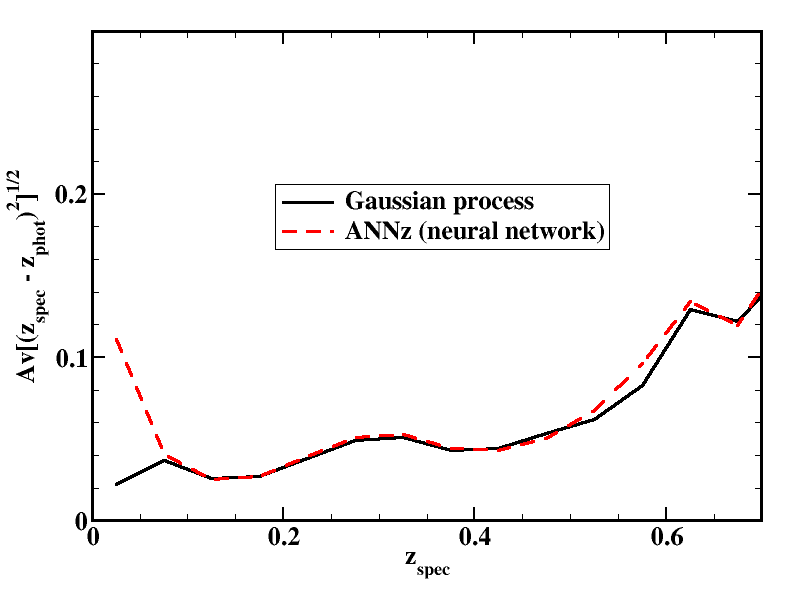
\includegraphics[scale=0.25]{dz_fig_kk200.png}
\label{dzfiga}
}
\subfigure[]{
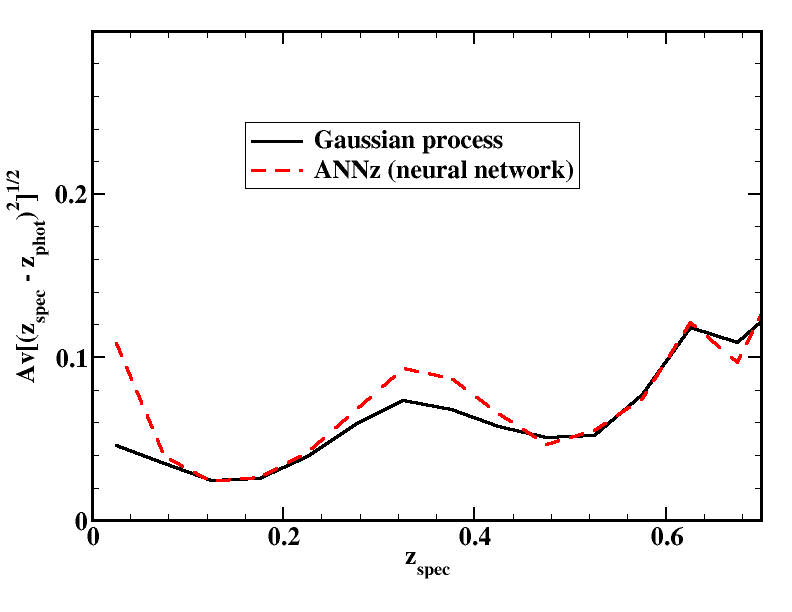
\includegraphics[scale=0.25]{dz_fig_gap_kk200.png}
\label{dzfiggap}
}}
\caption{
The square root of the sample mean of $(z_\text{spec}-z_\text{phot})^2$
as determined by a Gaussian process with covariance function (\ref{testcovar})
and the neural network code ANNz \cite{annz}.  Figure \ref{dzfiga} uses the
entire data set as described in the text.  Figure \ref{dzfiggap} shows the
results when all galaxies with $0.2\le z\le0.4$ are removed from the training and
validation sets.
}
\label{dzfig}
\end{figure}

We propose to build algorithms that are not only robust against incomplete
data, but are able to extrapolate photometric redshifts beyond the redshift
range of the training data.  We will incorporate measurement errors into
the inputs of the Gaussian process and propagate them through to the
photometric redshift in a self-consistent way.  The algorithms will be
trained and tested on simulated and existing data sets.  Simulated data
will be drawn from the LSST simulations which incorporate variations in
photometry due to extinction, galactic reddening, photometric calibration,
and sky background (including the associated uncertainties).  Connolly is
the LSST lead for simulation.  Validation of these techniques will utilize
existing data sets comprising spectroscopic redshifts and five band
photometry for one million galaxies taken from the SDSS (for low redshift
galaxies) and 30,000 galaxies from the
DEEP2\footnote{http://deep.ps.uci.edu} survey (for high redshift galaxies).
We will extend these datasets to include multiple narrow band observations
to evaluate how well we can measure redshifts with narrow band photometry.
We will assess the performance of our algorithms by minimizing both the
mean bias $\text{Av}[z_\text{spec}-z_\text{phot}]$ of determined photometric
redshift and their RMS scatter (the vertical axis of Figure \ref{dzfig}).

\subsection{Active Learning and Photometric Redshifts}
\label{sec:mlpz}

The discussion above illustrates how the appropriate choice of machine
learning algorithm can affect the fidelity of one's photometric redshift
determinations.  Further gains can be made if one is similarly judicious in
choosing a training set.  While next generation surveys like the LSST will
be exclusively photometric, they will present us with large numbers of
galaxies which we will have the option to follow-up with off-site
spectroscopy.  It behooves us, therefore, to develop a quantitative way of
determining which galaxies represent the most effective use of these
limited follow-up resources.  Such methods fall in the field of active
learning and we will develop novel algorithms for this purpose.

Active learning algorithms iteratively decide which data points they will
collect outputs on and add to the training set.  The goal is to choose the
points that will most improve the model being learned.  At each step, they
consider the current training data, the potential training data that could
be collected, and the current learned model, and evalute each potential new
point according to some objective criterion.  After selecting one or more
new points, the outputs for those points are collected and added to the
training set and the process repeats.  The key to the active learning
algorithm is the specification of the objective criterion used for
selection.  Settles (2009) presents a survey of such criteria.

We illustrate the potential impact of active learning in Figure
\ref{brentfig}, taken from Bryan (2007).  This figure considers the problem
of comparing the space of cosmological parameters (in this case, the
two-dimensional space of density due to matter $\Omega_m$ and density due
to cosmological constant $\Omega_\Lambda$) to supernova luminosity-distance
data \cite{essence}.  A 300$\times$300 test grid is drawn in parameter
space and the $\chi^2$ values on that grid are calculated.  The points that
lie within the 95\% confidence limit determined by the data are labeled to
provide a ground truth test set for learning algorithms. 
Three machine learning algorithms -- two driven by traditional Markov Chain Monte Carlo
(MCMC) methods, one driven by an active learner -- are set exploring parameter space to
learn the grid.
Traditional MCMC methods are shown by the blue and black curves.  The red
curve shows an active learner.  In Figure \ref{brentfig}, the horizontal
axis represents the number of training points sampled by the learners.  The
vertical axis represents the fraction of gridpoints that are misclassified
by the algorithms.
The active learner-guided algorithm converges to effectively 100\% accuracy
orders of magnitude faster than the traditional MCMC methods.  For similar
work demonstrating the efficacy of active learning, see also Bryan {\it et
  al}. (2007) and Daniel {\it et al}. (2012).

\begin{figure}[t]
\centerline{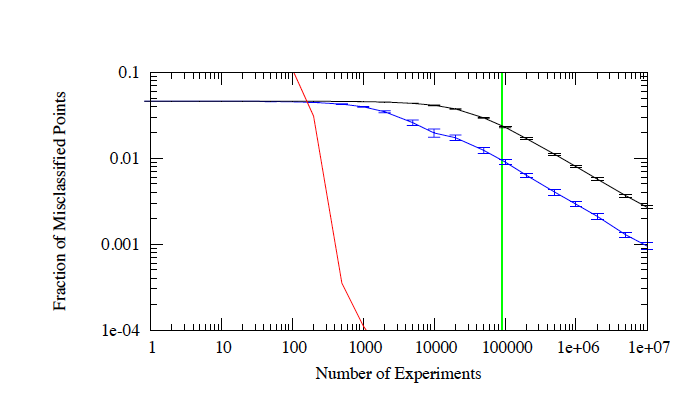
\includegraphics[scale=0.4]{apsvmcmc.png}}
\caption{This figure, taken from Bryan (2007), demonstrates the ability of
  active learning to accelerate the learning of a classifier. See text for
  a detailed description. The blue and black curves reprsent a machine
  learner without active learning. The red curve represents active
  learning. The green vertical bar is the number of points in the test
  grid, thus indicating the number of samples that would be needed to
  simply sample the grid exhaustively. }
\label{brentfig}
\end{figure}

In the case of photometric redshifts, an active learner would
generate a list of galaxies for which follow-up telescopes
should take spectroscopic information.  In the case of transient
classification, the algorithm would direct observers in choosing which
candidates to observe through which filters when.

Consider the set of all galaxies for which we have photometric observations
but no spectra, and thus no ``ground truth'' redshifts.  We will refer to
them with superscript $t$ and call them ``test points.'' With the training
data we do have, we can use Gaussian processes to estimate the mean and
covariance of these unknown redshifts as in equations (\ref{eq:mean}) and
(\ref{eq:cov}).  A classic active learning method, called uncertainty
sampling, uses the uncertainty of each test point as the criterion and
chooses the most uncertain point, which is the point corresponding to the
largest diagonal element of $\Sigma^{t}$, for spectroscopy.  With a Gaussian process,
however, it is easy to evaluate a ``one-step look ahead'' criterion.

Observe that while the mean predicted redshift for each test point is a
weighted combination of the observed redshifts in the training set, the
covariance does not depend on the observed redshifts.  Therefore, it is
easy to compute what the resulting covariance for the remaining test set
will be after observing the redshift for a point $q$ and moving that point
from the test set to the training set.  We refer to that covariance as
$\Sigma^{t|q}$.  We propose two objective criteria for active learning both
based on $\Sigma^{t|q}$.  The first is $\text{tr}(\Sigma^{t|q})$, where
$\text{tr}(A)$ indicates the trace of $A$.  This computes the sum of the
variances of the test points and the active learning algorithm chooses the
point $q$ that minimizes this quantity.  This method corresponds to
V-optimality in optimal experiment design and makes sense intuitively.  Our
ultimate goal is to reduce the uncertainty over our entire set of observed
galaxies and this criterion does so directly.  It is not optimal because
the sequential greedy selection of points may not choose the same points as
one that optimally chooses an entire set of observations in one shot and
doing the latter is computationally intractable.  However, our recent
results on submodularity and others suggest it may be close to optimal
\cite{YifeiMa12}.

We propose an additonal, more novel method.  We recently considered the
problem of optimal surveying (polling) \cite{Garnett12}.  Rather than
having a goal of correctly predicting the output for each point in a test
set, the goal is to predict the average output (or the class proportions in
classification problems) over the test set.  The estimate is simply the
average of the vector form of eq. (\ref{eq:mean}) and its variance is
proportional to the sum of all the elements of $\Sigma^{t|q}$.  In
preliminary experiments on graphs and other domains, minimizing this survey
variance not only performs well on the surveying problem, but also
outperforms the trace criterion and other popular active learning methods
such as uncertainty and density sampling \cite{activelearning} on active
learning problems.  Intuitively, it seems reasonable that considering the
entire covariance matrix might lead to better performance than choosing
only based on its diagonal.  We have little theoretical understanding of
why this is better than the trace criterion which directly optimizes the
quantity on which we will ultimately measure performance.  We will seek a
better theoretical understanding of this phenomenon as part of this work.

We will evaluate both of these methods in a standard simulated active
learning test.  This is done with a data set where all redshifts are
available.  Initially, they are all hidden from the active learner and they
are only revealed as the learner ``queries'' those points.  The performance
of the active learning algorithm is evaluated at each step of the process
by measuring the total error of its predictions on the data points it has
not yet queried.  We will draw our data both from simulations of the expected
data from the LSST \cite{imsim} and from existing survey data,
including those that are complete as a function of magnitude (e.g. SDSS) and
those with known selection biases (e.g. DEEP2).  The final goal of this
component of the proposal will be to predict spectroscopic
redshifts which, if obtained, will
improve the performance of photometric redshift algorithms.  Intially, we will
use our results to acquire multiple narrow band photometric observations that
will act as a proxy for spectroscopic observations \cite{narrow}.
We will then address the question of supplementing the DEEP2 
spectroscopic observations to
define a training sample adequate for the photometric redshift needs of the Dark
Energy Survey and LSST projects.


We note that spectroscopic survey campaigns for faint galaxy samples
can take many years to complete.  With first light on the LSST less
than a decade away, we must lay the groundwork now if the desired
cosmological results are to be achieved in a reasonable amount of
time.


\section{Transient Classification}
\label{sec:transient}

Real-time automatic classification of objects is already widely acknowledged as a
necessary support technology for the forthcoming age of survey astronomy
\cite{djorgovski2011,richards2011,richards2012,graham2012,mahabal2008a,mahabal2011a}.
Objects will need to be categorized into known science classes so that novel
or rare objects can be flagged for detailed follow-up observations.
For transient events, algorithms must be able to make rapid
decisions so that sources can be targeted for follow-up 
and classifications learned before
objects return to their quiescent phases.  A great deal of work has
already been done developing algorithms that can learn the classification of an
object given a fixed set of observations and training data.  
Mahabal {\it et al}. (2008a,2011a,2011b) propose to break down the
observations of a given object into $\{\Delta m,\Delta t\}$ pairs (where $m$
is magnitude and $t$ is time) and use the density of observations in this 
two-dimensional space as the basis for a Bayesian classification algorithm.
Mahabal {\it et al}. (2008b) alternatively propose to use those same 
$\{\Delta m,\Delta t\}$ pairs as the input to a Gaussian process regression
by which they will reconstruct the object's entire light curve as a function
of time, and then classify the object based on that reconstruction.
Richards {\it et al}. (2011) use observations of transient objects to extract
periodic (e.g. the amplitude and frequency of the first two Fourier modes of
the object's light curve) and non-periodic (e.g. the variance and skewness of
all of the magnitude observations taken, regardless of their separation in
time) and feed those features into several tree-based classifiers.
They find misclassification rates lower than 30\% with their best method yielding a
misclassification rate of 22.8\%.  Using only non-periodic features, which will be
especially easy for survey telescopes to gather, rather than
full light curves, they 
find a misclassification rate of
between 26\% and 28\%.
Bloom {\it et al}. (2011) also use a tree-based automatic classifier on
Palomar Transient Factory data and find a 3.8\% error rate when
discriminating between four major classifications.  Richards {\it et al}.
consider a more complete set of 25 possible classifications.
Clearly, many possibile approaches are available for the automated
classification of transient objects, and not all of them rely upon highly
detailed observations to function.

While significant attention has been paid to the problem of classifying an
object once training sets and observations have been assembled, relatively
little has been paid to optimizing the training set or observations.
Though the budgeted observing programs of survey telescopes leave little
time to follow-up serendipitous discoveries, other telescopes will be much
freer to fill in the gaps in survey-derived knowledge.  The question is
how best to do so.  The problem of sub-optimal training data is already being
faced by the community.  Figure 6 of Richards {\it et al}. (2011)
demonstrates that automated classifiers are much better at identifying
objects of common types, for which training data is abundant, than they are
at identifying objects of rare types, for which training data is sparse.
The authors address this problem in Richards {\it et al.} (2012) by designing
an active learning algorithm which selectively adds to the training set,
choosing objects of uncertain classification and asking human classifiers to
provide detailed information (via either their expertise alone or with
follow-up observations) about the queried object.  They find that this scheme
reduces the misclassification rate 
of their classifier by approximately five percentage
points over a scheme which randomly constructs its training data set (see
their Figure 6).

This work demonstrates the potential of integrating active
learning into survey astronomy, however it does not 
account for the importance of
generating further 
observations about a source or the cost of these observations.  
The active learner implemented by
Richards {\it et al.} (2012)
simply asks its human operators to provide classifications without offering
any guidance how.  Certainly, the humans would be almost guaranteed to
find the proper classification if they were to take both a full spectrum
and light curve of
the source, but this would come at the expense of a great deal of time and
effort.  We propose to eliminate this burden by using active learning not
only to designate objects to be added to the training set, but to designate
observations of those objects that would be the most efficient.  Figure 8 of
Richards {\it et al}. (2011) and Figure 13 of Bloom {\it et al}. (2011)
demonstrate that, for different classes of objects, different features are
more or less important.  If the machine learner already has an idea to what
class the queried object belongs, it should be able to give the operator a
recommendation of what observation to perform.  Maybe only a few color
measurments are needed to determine the object's physical origin.  
Maybe observations at only a few select epochs, rather than a drawn out time
series, will be needed to infer the object's complete light curve.
Maybe the required observations are consistent with the survey telescope's 
existing schedule, and no special follow-up will be required at all.  In this
way, active learning will allow us not only to maximize the science output of
our surveys, but to do so with the most efficient allocation of resources,
ensuring that we gain the most information about the most objects with the
least time and effort.

We will evaluate these approaches using simulated data from the LSST
\cite{imsim} which incorporates transient and variable sources, as well as
existing data streams from the SDSS (with 70+ epochs of observations) and
LINEAR\footnote{http://www.ll.mit.edu/mission/space/linear} \cite{linear}.
Many of the present attempts at automatic transient classification
draw their training sets from different surveys than their test sets.  
Long {\it et al}. (2012) find that this heterogeneity can degrade the quality of
the classifications significantly.  Their Figure 1 shows how the
misclassification rate of a classifier trained on Hipparcos data goes from 0.6\%
when tested against other Hipparcos data to 30\% when tested against OGLE data. 
If we are to develop algorithms which are useful on the LSST, we must work with
simulated data that is representative of what we expect from the LSST's actual
performance.  

\subsection{Active Learning for Transient Objects}

The input features for transient object classification will be photometric
and morphologic measures taken at different increments in time.  The output
is a categorical variable indicating the class.  This is in contrast to
photometric redshifts where the output is continuous.  Fortunately, the
underlying covariance for Gaussian process classification is the same as
for regression and we will adopt a similar prediction model.

The active learning problem for transient objects contains three
subproblems, active learning, active search, and active feature
acquisition.  Finally, one additional difference between the transient
object method and the photometric redshift method is that transient object
decisions must be made in an online, streaming fashion.  Rather than
considering an entire pool of test objects, they appear one at a time as
they are detected and the algorithm must decide whether and how to follow
up on each immediately as they are detected.  We first describe algorithms
for each of the three pieces and then how to combine them into a single
algorithm for streaming transient detections.

{\bf Active Learning.} In order to get a ground-truth class for a transient
object, repeated observations are taken to estimate a full light curve.  A
human expert then assigns a class label.  Both the repeated telescope
observations and human time are expensive and thus we want to learn a good
classification model using limited training data.  We propose a
corresponding trace and survey criteria for active learning on transients
as in Section \ref{sec:mlpz}.

{\bf Active Feature Acquisition.} When considering photometric redshifts,
we assumed that all photometric inputs were observed for every object of
interest.  For transients this will not be the case.  A large component of
the problem is deciding for each object, whether observations of additional
colors and/or additional times would be valuable in classifying or
characterizing the object.

We propose to extend our recent work on using GPs to detect damped
lyman-alpha (DLA) systems \cite{Garnett12a}.  In that work GP regression
was used on each observed, noisy spectrum to infer the latent spectrum.
The single independent (input) variable was wavelength.  For transient
objects we will have 5 color magnitudes that are a function of time and are
coupled to each other.  In the DLA work, a different model was learned for
spectra with and without a DLA.  DLAs were classified by recognizing which
model fit best.  In the proposed work, we will learn a different model for
each class of object and will estimate class probabilities using Bayes rule
for combining the prior probability for each class and how well the
respective models fit the observations.  The key advantage of this approach
is that the GPs naturally provide a mean and covariance for future
unobserved colors.  This uncertainty propagates through to class labels and
we can use it to estimate the reduction in class uncertainty that will be
gained by observing a certain color at a certain time.  The observation
yielding the greatest reduction in entropy for the class and the light
curves for this object will be taken.

{\bf Active Search.} Many transient objects will be from common and/or 
well-understood classes that do not have much observational value.  The ultimate
objective in following up detected transients is to maximize the number of
interesting transients classified and characterized while staying within a
budget of follow-up observations.  This is an active search problem. The
problem and the Bayesian optimal algorithm for it are described in our
recent work \cite{Garnett11,Garnett12}.  As in active learning, the
acquisition of class labels is expensive and we need to learn a model to
predict these labels from limited input data.  However, the final
performance objective is not the accuracy of the classifier, but rather the
number of positives (i.e. objects from interesting classes) identified.  We
propose to use the simple myopic algorithm described in that work.  It
computes the probability of each point belonging to the positive class and
chooses the largest.


{\bf A combined streaming method.} The three goals above will be combined
in a staged set of decisions.  When a new transient is detected, the light
curve model will be used to provide estimated light curves for the object.
Those light curves are the input variables for this object in the active
learning and active search algorithms.  In parallel, the active learning
and active search methods will decide whether to follow up on this object.
If either of them selects the object, it is advanced to active feature
acquisition.  There additional observations on the object are selected and
the process for this object repeats.  An object that initially seemed
interesting to one algorithm may cease to be so after additional
observations or may be adopted by the other one.  The process for one
object terminates when neither active learning nor active search remains
interested in it or the object class and light curves are characterized
well enough that no more observations are required.

The active search and active learning algorithms each compute an objective
criterion score for each object.  For photometric redshifts the scores are
used to create a ranked list and observations are scheduled proceeding down
the list.  When a budget is given for follow-ups on each batch of newly
detected transients, going down a ranked list in each batch until that
budget is exhausted is appropriate.

However, when the budget is an aggregate over a longer time period a
streaming decision on how much of the budget to spend on each batch must be
made on that batch in isolation.  This will be done by choosing a score
threshold.  The threshold will be set by evaluating the historical stream
and setting it at a value that would yield a number of follow ups equal to
an available budget for following up.  The threshold will be adjusted
continuously as more observations are taken and the models and scientific
goals change (e.g. the object types designated as ``interesting'' are
changed).

Since all of the algorithm components are based on GP models, it is
possible to merge them together into a single model.  We hypothesize that
additional performance improvements can be made through an integrated model
and decision algorithm.  For example, an object with a modest active
learning score that can be easily characterized with only one more follow
up might be promoted over one with a higher score that can not be easily
characterized even with many more observations.  After we have implemented
the staged method described above, we will investigate and compare an
integrated model.

\section{Results of Prior NSF Support}

Connolly, Schneider, and Daniel are all part of an active
collaboration between computer scientists, statisticians and
astrophysicists at Carnegie Mellon University and the University of
Washington.  This collaboration, dating to 2001, has demonstrated
sustained success and was cited by the President of the American
Statistical Association (ASA) as an exemplary interdisciplinary
research team \cite{straf03}. Highlights from this collaboration
include n-tree searching algorithms that make the calculation of
n-point correlation functions scale to size of current surveys
\cite{Moore00}. This software was made publicly available and has been
used to compute the 2--point function on over 10$^6$ galaxies and the
3--point correlation function of 400,000 galaxies from the SDSS survey
\cite{Scranton2002,Szapudi2002,Nichol2006,mcbride2011a,mcbride2011b}
as well as in measures of the marked correlation functions
\cite{Skibba2006}.  As part of this collaboration \cite{yip2004a,
  vdp2009, daniel2011} introduced signal compression and analysis
techniques to astronomy that are now regularly applied to the analysis
of current spectroscopic surveys.

Schneider heads a machine learning group that has done extensive work
on automatic anomaly detection and pattern-recognition in complex data
sets \cite{Xiong2011gad,poczos12CVPR}.  Connolly leads the catalog and
image simulation effort for the LSST. He developed the simulations and
analyses that were used to predict the photometric redshift
performance of the LSST as well as the dependence of photometric
redshifts on the LSST characteristics (including filter complement and
filter shapes). Daniel has developed techniques used in active
learning, dimensionality reduction, and theoretical cosmology
\citep{daniel2011, daniel2012}.

The authors have spent the last two years working on grants from the
National Science Foundation and the Department of Energy to apply
methods from machine learning to astrophysical problems.  This work
has resulted in papers demonstrating the ability of computer
algorithms to automatically classify astronomical objects
\cite{vdp2009,daniel2011} as well as a paper using simplified active
learning methods to accelerate the exploration of complex parameter
spaces \cite{daniel2012}.  Connolly's most recent NSF award IIS-0844580
\$490,398 ``Putting Astronomy's Head in the Cloud'' (2009 -- 2012) led
to the development of scalable image analysis tools that are built
upon the Hadoop platform\citep{wiley2011}. Schneider's NSF Award
0911032 (co-PI), ``III: Large: Discovering Complex Anomalous Patterns'',
2009-2013, funds a collaboration of computer scientists and medical
doctors to identify complex patterns in medical care data. As part of
this work he developed several new methods of regularization to learn
complex models with only a small amount of training data
\cite{YiZhangICML2010,YiZhangSDM2010,YiZhangMultitask2010,YiZhang2011multiECOC,YiZhang2012},
for non-parametric estimators for divergences and dependencies
\cite{poczos11alphadiv,Poczos2011UAI,poczos12CVPR}, and for graphical
models for finding groups of collectively anomalous records
\cite{Xiong2011gad,xiong2011fgm}.

Beyond the computational and astrophysical aspects of this research
the PIs have demonstrated a commitment to developing and releasing
applications for data intensive cosmology and for integrating research
and education (see, for example, the extensive machine learning tools
available at http://www.autonlab.org/autonweb/downloads/software.html
and the python tools for astronomical analyses at  http://astroml.github.com). In the field of
informal education, Connolly was the technical lead for the development
of Sky in Google Earth (Google Sky; http://earth.google.com) which
enabled the seamless exploration of astronomical images of the sky, and
recently developed an affordable digital planetarium system using
Microsoft's World Wide Telescope software \cite{rosenfield2011}.

All tools and codes developed through this program will be open-source
and made available on the web. The resulting framework will be tested
on relevant datasets including the SDSS observations and the LSST
simulations, whose results will be pipelined into an online database
with public access.





\section{Broader Impacts}
\label{sec:broad}

The algorithms developed for determining photometric redshift will immediately
find use constructing data sets to constrain cosmological theories through both
the weak lensing correlation function and the three-dimensional galaxy-galaxy
correlation function.  
They will play important roles in the attempts by 
the Dark Energy Survey, EUCLID, and LSST to constrain dark energy.
The algorithms developed for transient classification
will help researchers to deal with the transient alert streams from surveys like
the LSST, the Palomar Transient Factory, and the Catalina Sky Survey.  
Automated identification of
interesting objects will help prevent researchers from being overwhelmed by a
flood of mundane objects that do not warrant further observation.
These algorithms will also provide important guidance to constructing follow-up
facilities optimized to classify the transient and variable sources observed by
large surveys.

The algorithms developed by this project will also 
find application in citizen astronomy through the framework
of the Zooniverse\footnote{https://www.zooniverse.org}.  
The crowd sourcing of galaxy
classification has already allowed
scientists to classify more and more diverse objects faster than was
previously possible.  
Crowd sourcing algorithms driven by active learning principles will be
able to make more efficient use of human resources, ensuring that humans are
shown only the most interesting, difficult to parse objects.  Machine learning
algorithms coupled to crowd sourced data will be able to learn more than any
algorithms before them, giving more precise inferences on data in less time than
could be accomplished by algorithms trained by a single scientist or research
group.  We will provide versions of our algorithms for interface with the
Zooniverse infrastructure to optimally leverage human expertise in preparing for
the next generation of surveys.

Thinking beyond the next generation of surveys, the integration of active
learning algorithms into astronomy will help funding agencies and advisory
panels to determine what is the best next step for the community to take.  Just
as the NSF's Dark Energy Task
Force\footnote{http://www.nsf.gov/mps/ast/detf.jsp} focused the disparate
attentions of the cosmological community on maximixing the $\{w,w_a\}$ Figure of
Merit of future experiments, future panels will be able to use the quantifiable
information gains predicted by active learning to determine how to evaluate
competing science priorities beyond the next decade.

If astronomy is to remain a window on ``the most profound mysteries in all of
science'' (the way Michael Turner once described dark energy), it must be
prepared to deal with large data in a quantifiable and robust way.  Machine and
active learning provide that facility.  We propose the above research program as
a means of integrating these methods into the field.

\newpage
%%%%%%%%%%%%%%%%%%%%%%%%%%%%%%%%%%%%%%%%%%%%%%%%%%%%%%%%%%%%
%%%%%%%%%%%%%%%%%%%%%%%%%%%%%%%%%%%%%%%%%%%%%%%%%%%%%%%%%%%%

%%%%%%%%%%%%%%%%%%%%%%%%%%%%%%%%%%%%%%%%%%%%%%%%%%%%%%%%%%%%
%%%%%%%%%%%%%%%%%%%%%%%%%%%%%%%%%%%%%%%%%%%%%%%%%%%%%%%%%%%%
\begin{thebibliography}{99}

\bibitem[Abazajian {\it et al}. 2009]{Abazajian:2008wr}
  Abazajian, K.~N.{\it et al.}  [SDSS Collaboration]~2009,
  %``The Seventh Data Release of the Sloan Digital Sky Survey,''
  The Astrophysical Journal Supplement Series  {\bf 182}, 543
  [arXiv:0812.0649 [astro-ph]].
  %%CITATION = APJSA,182,543;%%

\bibitem[Abdalla {\it et al}. 2011]{abdalla}
Abdalla,~F.~B., Banerji,~M., Lahav,~O., and Rashkov,~V. 2011,
Monthly Notices of the Royal Astronomical Society {\bf 417}, 1891

\bibitem[Abramo {\it et al}. 2012]{narrow}
Abramo,~L.~R., Strauss,~M.~A., Lima,~M., Hern\'andez-Monteagudo,~C., Lazkoz,~R.,
Moles,~M., de Oliveira,~C.~M., Sendra,~I., Sodr\'e Jr.,~L., and
Storchi-Bergmann,~T. 2012, Monthly Notices of the Royal Astronomical Society
{\bf 423}, 3251

\bibitem[Albrecht {\it et al}. 2006]{detf}
Albrecht,~A., Bernstein,~B., Cahn,~R., Freedman,~W.~L., Hewitt,~J.,
Hu,~W., Huth,~J., Kamionkowski,~M., Kolb,~E., Knox,~L., Mather,~J.~C.,
Staggs,~S., Suntzeff,~N.~B. (Dark Energy Task Force) 2006,
``Report of the Dark Energy Task Force,''
\verb|http://jdem.gsfc.nasa.gov/science/DETF_Report.pdf|


\bibitem[Berg\'e {\it et al}. 2012]{psf}
Berg\'e,~J., Price,~S., Amara,~A., and Rhodes,~J. 2012,
Monthly Notices of the Royal Astronomical Society {\bf 419}, 2356

\bibitem[Bloom {\it et al}. 2011]{bloom2011}
Bloom,~J.~S., Richards,~J.~W., Nugent,~P.~E., Quimby,~R.~M., Kasliwal,~M.~M.,
Starr,~D.~L., Posnanski,~D., Ofek,~E.~O., Cenko,~S.~B., Butler,~N.~R.,
Kulkarni,~S.~R., Gal-Yam,~A., and Law,~N. 2011 [arXiv:1106.5491]

\bibitem[Bonfield {\it et al}. 2010]{Bonfield}
Bonfield,~D.~G., Sun,~Y., Davey,~N., Jarvis,~M.~J., Abdalla,~F.~B.,
Banerji,~M., Adams,~R.~G. 2010, Monthly Notices of the Royal Astronomical Society 
{\bf 405} 987

\bibitem[Brammer {\it et al}. 2008]{eazy}
Brammer,~G.~B., van Dokkum,~P.~G., and Coppi,~P. 2008,
The Astrophysical Journal {\bf 686}, 1503

\bibitem[Bryan 2007]{brentsthesis}
Bryan, B., 2007, Ph.D. thesis
\verb|http://reports-archive.adm.cs.cmu.edu/anon/|
\verb|ml2007/abstracts/07-122.html|

\bibitem[Bryan {\it et al}. 2007]{bryan}
Bryan, B., Schneider, J., Miller, C.~J., Nichol, R.~C., Genovese, C., and
Wasserman, L., 2007,
The Astrophysical Journal {\bf 665}, 25

\bibitem[Budav\'ari 2008]{budavari2008}
Budav\'ari,~T. 2008 The Astrophysical Journal {\bf 695}, 747

\bibitem[Collister and Lahav 2004]{annz}
Collister,~A.~A. and Lahav,~O. 2004,
Publications of the Astronomical Society of the Pacific {\bf 116}, 345

\bibitem[Connolly {\it et al}. 2005]{imsim}
Connolly,~A.~J., Peterson,~J., Jernigan,~J.~G., Abel,~R., Bankert,~J.,
Chang,~C., Claver,~C.~F., Gibson,~R., Gilmore,~D.~K., Grace,~E., Jones,~R.~L.,
Ivezic,~Z., Jee,~J., Juric,~M., Kahn,~S.~M., Krabbendam,~V.~L., Krughoff,~S.,
Lorenz,~S., Pizagno,~J., Rasmussen,~A., Todd,~N. Tyson,~J.~A., and Young,~M.
2005, Society of the Photo-Optical Instrumentation Engineers (SPIE) Converence
Series {\bf 7738}, 53

\bibitem[Cunha {\it et al}. 2012]{cunha2012}
Cunha,~C.~E., Huterer,~D., Lin,~H., Busha,~M.~T., and Wechsler,~R.~H. 2012,
[arXiv:1207.3347]

\bibitem[Daniel and Linder 2010]{muvarpi2}
Daniel,~S.~F. and Linder,~E.~V. 2010, Physical Review D {\bf 82}, 103523

%\cite{Daniel:2011rr}
\bibitem[Daniel {\it et al}. 2011]{daniel2011} 
  Daniel,~S.~F., Connolly,~A.~J., Schneider,~J., Vanderplas,~J. and Xiong,~L. 
  %``Classification of Stellar Spectra with LLE,''
  The Astronomical Journal  {\bf 142}, 203 (2011)
  [arXiv:1110.4646 [astro-ph.SR]].
  %%CITATION = ARXIV:1110.4646;%%

\bibitem[Daniel {\it et al}. 2012]{daniel2012}
Daniel,~S.~F., Connolly,~A.~J., and Schneider,~J. 2012
[arXiv:1205.2708]

\bibitem[Das {\it et al}. 2011]{sudeep}
Das,~S., de Putter,~R., Linder,~E.~V., and Nakajima,~R. 2011,
[arXiv:1102.5090]

\bibitem[Davis {\it et al}. 2007]{essence}
Davis,~T.~M., M\"ortsell,~E., Sollerman,~J., Becker,~A.~C., Blondin,~S.,
Challis,~P., Clocchiatti,~A., Filippenko,~A.~V., Foley,~R.~J., Garnavich,~P.~M.,
Jha,~S., Krisciunas,~K., Kirshner,~R.~P., Leibundgut,~B., Li,~W., Matheson,~T.,
Miknaitis,~G., Pignata,~G., Rest,~A., Riess,~A.~G., Schmidt,~B.~P.,
Smith,~R.~C., Spyromilio,~J., Stubbs,~C.~W., Suntzeff,~N.~B., Tonry,~J.~L.,
Wood-Vasey,~W.~M., and Zenteno,~A. 2007, The Astrophysical Journal, {\bf 666},
716

\bibitem[de Putter {\it et al}. 2010]{roland}
de Putter,~R., Huterer,~D. and Linder,~E.~V. 2010, Physical Review D {\bf 81},
103513


\bibitem[Djorgovski {\it et al}. 2011]{djorgovski2011}
Djorgovski,~S.~J., Donalek,~C., Mahabal,~A.~A., Moghaddam,~B., Turmon,~M.,
Graham,~M.~J., Drake,~A.~J., Sharma,~N. and Chen,~Y. 2011
[arXiv:1110.4655] to appear in Statistical Analysis and Data Mining, ref. proc.
CIDU 2011 conf., eds. A. Srivastava and N. Chawla

\bibitem[Garnett {\it et al}. 2011]{Garnett11}
Garnett,~R., Krishnamurhty,~Y., Wang,~D., Schneider,~J., and Mann,~R. 2011,
``Bayesian Optimal Active Search on Graphs,'' KDD Workshop on Mining and
Learning with Graphs

\bibitem[Garnett {\it et al}. 2012a]{Garnett12}
Garnett,~R., Krishnamurthy,~Y., Xiong,~X., Schneider,~J., and Mann,~R. 2012a,
``Bayesian Optimal Active Search and Surveying,'' International Conference on
Machine Learning

\bibitem[Garnett {\it et al}. 2012b]{Garnett12a}
Garnett,~R., Ho,~S., and Schneider,~J. 2012b,
``Gaussian Processes for Identifying Damped Lyman-alpha Systems in Spectroscopic
Surveys,'' Neural Information Processing Systems 
workshop on Modern Nonparametric Methods in Machine Learning

\bibitem[Graham {\it et al}. 2012]{graham2012}
Graham,~M.~J., Djorgovski,~S.~G., Mahabal,~A., Donalek,~C., Drake,~A.,
Longo,~G. 2012 [arXiv:1208.2480] to appear in special issue of Distributed and
Parallel Databases on Data Intensive eScience

\bibitem[Huterer {\it et al}. 2006]{huterer2006}
Huterer,~D., Takada,~M., Bernstein,~G., and Jain,~B. 2006,
Monthly Notices of the Royal Astronomical Society {\bf 366}, 101

\bibitem[Kitching {\it et al}. 2008]{kitching}
Kitching,~T.~D., Taylor,~A.~N., and Heavens,~A.~F. 2008,
Monthly Notices of the Royal Astronomical Society {\bf 389} 173

\bibitem[Long {\it et al}. 2012]{long2012}
Long,~J.~P., El Karoui,~N., Rice,~J.~A., Richards,~J.~W., and Bloom,~J.~S. 2012,
Publications of the Astronomical Society of the Pacific {\bf 124} 280

\bibitem[LSST Collaboration 2011]{lsstoverview}
LSST Collaboration 2011, [arXiv:0805.2366]
\verb|http://www.lsst.org/lsst/overview/|

\bibitem[LSST Dark Energy Science Collaboration 2012]{desc}
LSST Dark Energy Science Collaboration 2012, [arXiv:1211.0310]

\bibitem[LSST Science Collaborations 2009]{sciencebook}
LSST Science Collaborations 2009, ``LSST Science Book'',
\verb|http://www.lsst.org/lsst/science/scibook|

\bibitem[Ma {\it et al}. 2006]{Ma2006}
Ma,~Z., Hu,~H., and Huterer,~D. 2006, The Astrophysical Journal {\bf 636}, 21

\bibitem[Ma {\it et al}. 2012]{YifeiMa12}
Ma,~Y., Garnett,~R., and Schneider,~J. 2012,
``Submodularity in Batch Active Learning and Survey Problems
on Gaussian Random Fields,''
Neural Information Processing Systems 
workshop on Discrete Optimization in Machine Learning

\bibitem[Mahabal {\it et al}. 2008a]{mahabal2008a}
Mahabal,~A., Djorgovski,~S.~G., Turmon,~M., Jewell,~J., Williams,~R.~R.,
Drake,~A.~J., Graham,~M.~G., Donalek,~C., Glikman,~E., and the Palomar-QUEST Team
2008a, Astronomische Nachrichten {\bf 329}, 288

\bibitem[Mahabal {\it et al}. 2008b]{mahabal2008b}
Mahabal,~A., Djorgovski,~S.~G., Williams,~R., Drake,~A., Donalek,~C.,
Graham,~M., Moghaddam,~B., Turmon,~M., Jewell,~J., Khosla,~A., and
Hensley,~B. 2008b [arXiv:0810.4527] to appear in proceedings fo the Class2008
conference (Classification and Discovery in Large Astronomical Surveys, Ringberg
Castle, 14-17 October 2008)

\bibitem[Mahabal {\it et al}. 2011a]{mahabal2011a}
Mahabal,~A.~A., Donalek,~C., Djorgovski,~S.~J., Drake,~A.~J.,
Graham,~M.~J., Williams,~R., Chen,~Y., Moghaddam,~B., and Turmon,~M.
2011a, [arxiv:1111.3699] to appear in Proc. IAU 285, ``New Horizons in Transient
Astronomy,'' Oxford, September 2011

\bibitem[Mahabal {\it et al}. 2011b]{mahabal2011b}
Mahabal,~A.~A., Djorgovski,~S.~G., Drake,~A.~J., Donalek~C., Graham,~M~J.,
Williams,~R.~D., Chen,~Y., Moghaddam,~B., Turmon,~M., Beshore,~E., and Larson,~S.
2011b, Bulletin of the Astronomical Society of India {\bf 39}, 387

\bibitem[Mandelbaum {\it et al}. 2008]{mandelbaum2008}
Mandelbaum,~R., Seljak,~U., Hirata,~C.~M., Bardelli,~S., Bolzonella,!M.,
Bongiorno,~A., Carollo,~M., Contini,~T., Cunha,~C.~E., Garilli,~B.,
Iovino,~A., Kambczyk,~P, Kneib,~J.-P., Knobel,~C., Koo,~D.~C., Lamareille,~F.,
Le F\`evre,~O., Leborgne,~J.-F., Lilly,~S.~J., Maier,~C., Mainieri,~V.,
Mignoli,~M., Newman,~J.~A., Oesch,~P.~A., Perez-Montero,~E., Ricciardelli,~E.,
Scodeggio,~M., Silverman,~J., and Tasca,~L. 2008, Monthly Notices of the Royal
Astronomical Society {\bf 386}, 781

\bibitem[McBride {\it et al}. 2011a]{mcbride2011a}
McBride,~C.~K., Connolly,~A.~J., Gardner,~J.~P., Scranton,~R., Newman,~J.~A.,
Scoccimarro,~R., Zehavi,~I., and Schneider,~D.~P. 2011a, The Astrophysical
Journal, {\bf 726}, 13

\bibitem[McBride {\it et al}. 2011b]{mcbride2011b}
McBride,~C.~K., Connolly,~A.~J., Gardner,~J.~P., Scranton,~R., Scoccimarro,~R.,
Berlind,~A.~A., Mar\'in,~F., and Schneider,~D.~P. 2011b, The Astrophysical
Journal {\bf 739}, 85

\bibitem[Moore {\it et al}. 2000]{Moore00}
Moore,~A., Connolly,~A., Genovese,~C., Grone,~L., Kanidoris,~N., Nichol,~R.,
Schneider,~J., Szalay,~A., Szapudi,~I., and Wasserman,~L. 2000,
``Fast Algorithms and Efficient Statistics: N-point Correlation Functions,'' in
MPA/MPE/ESO Conference on Mining the Sky [arXiv:astro-ph/0012333]

\bibitem[Nakajima {\it et al}. 2012]{nakajima2011}
Nakajima,~R., Mandelbaum,~R., Seljak,~U., Cohn,~J.~D., Reyes,~R., and
Cool,~R. 2012, Monthly Notices of the Royal Astronomical Society {\bf 420}, 3240
[arXiv:1107.1395]

\bibitem[Nichol {\it et al}. 2006]{Nichol2006}
Nichol,~R.~C., Sheth,~R.~K., Suto,~Y., Gray,~A.~J., Kayo,~I., Wechsler,~R.~H.,
Marin,~F., Kulkarni,~G., Blanton,~M., Connolly,~A.~J., Gardner,~J.~P., Jain,~B.,
Miller,~C.~J., Moore,~A.~W., Pope,~A., Pun,~J., Schneider,~D., Schneider,~J.,
Szalay,~A., Szapudi,~I., Zehavi,~I., Bahcall,~N.~A., Csabai,~I., Brinkmann,~J.
2006, Monthly Notices of the Royal Astronomical Society {\bf 368}, 1507

\bibitem[Poczos and Schneider 2011]{poczos11alphadiv}
Poczos,~B. and Schneider,~J. 2011, ``On the Estimation of alpha-Divergences,''
Artificial Intelligence and Statistics (AISTATS)

\bibitem[Poczos {\it et al}. 2011]{Poczos2011UAI}
Poczos,~B., Xiong,~L., and Schneider,~J. 2011, ``Nonparametric Divergence Estimation with
Applications to Machine Learning on Distributions,''  Uncertainty in Artificial
Intelligence

\bibitem[Poczos {\it et al}. 2012]{poczos12CVPR}
Poczos,~B., Xiong,~L., Sutherland,~D., and Schneider,~J. 2012,
``Nonparametric Kernel Estimators for Image Classification,''
IEEE Conference on Computer Vision and Pattern Recognition

\bibitem[Rasmussen and Williams 2006]{gp}
Rasmussen, C.~E. and Williams, C.~K.~I., 2006, ``Gaussian
Processes for Machine Learning''
\verb|http://www.GaussianProcess.org/gpml/|

\bibitem[Richards {\it et al}. 2004]{qso}
Richards,~G.~T., Nichols,~R.~C., Gray,~A.~G., Brunner,~R.~J., Lupton,~R.~H.,
Vanden Berk,~D.~E., Chong,~S.~S., Weinstein,~M.~A., Schneider,~D.~P.,
Anderson,~S.~F., Munn,~J.~A., Harris,~H.~C., Strauss,~M.~A., Fan,~X.,
Gunn,~J.~E., Ivezi\'c,~Z., York,~D.~G., Brinkmann,~J., and Moore,~A.~W. 2004,
The Astrophysical Journal Supplement Series, {\bf 155}, 257

\bibitem[Richards {\it et al}. 2011]{richards2011}
Richards,~J.~W., Starr,~D.~L., Butler,~N.~R., Bloom,~J.~S., Brewer,~J.~M.,
Crellin-Quick,~A., Higgins,~J., Kennedy,~R., and Rischard,~M. 2011,
The Astrophysical Journal {\bf 733}, 10

\bibitem[Richards {\it et al}. 2012]{richards2012}
Richards,~J.~W., Starr,~D.~L., Brink,~H., Miller,~A.~A., Bloom,~J.~S.,
Butler,~N.~R., James,~J.~B., Long,~J.~P., and Rice,~J. 2012
The Astrophysical Journal {\bf 774}, 192

\bibitem[Rosenfield {\it et al}. 2011]{rosenfield2011}
Rosenfield,~P., Connolly,~A., Fay,~J., Sayres,~C., and Tofflemire,~B. 2011,
Astronomical Society of the Pacific Conference Series {\bf 443}, 109

\bibitem[Scranton {\it et al}. 2002]{Scranton2002}
Scranton,~R., Johnston,~D., Dodelson,~S., Frieman,~J.~A., Connolly,~A.,
Eisenstein,~D.~J., Gunn,~J.~E., Hui,~L., Jain,~B., Kent,~S., Loveday,~J.,
Narayanan,~V., Nichol,~R.~C., O'Connell,~L., Soccimarro,~R., Sheth,~R.~K.,
Stebbins,~A., Strauss,~M.~A., Szalay,~A.~S., Sapudi,~I., Tegmark,~M.,
Vogeley,~M., Zehavi,~I., Annis,~J., Bahcall,~N.~A., Brinkman,~J., Csabai,~I.,
Hindsley,~R., Ivezic,~Z., Kim,~R.~S.~J., Knapp,~G.~R., Lamb,~D.~Q., Lee,~B.~C.,
Lupton,~R.~H., McKay,~T., Munn,~J., Peoples,~J., Pier,~J., Richards,~G.~T.,
Rockosi,~C., Schlegel,~D., Schneider,~D.~P., Stoughton,~C., Tucker,~D.~L.,
Yanny,~B., York,~D.~G. 2002, The Astrophysical Journal {\bf 579}, 48

\bibitem[Sesar {\it et al}. 2011]{linear}
Sesar,~B., Stuart,~J.~S., Ivezi\'c,~\u Z., Morgan,~D.~P., Becker,~A.~C., and
Wo\'zniak,~P. 2011, The Astronomical Journal {\bf 142}, 190

\bibitem[Settles 2009]{activelearning}
Settles,~B. 2009, ``Active Learning Literature Survey,'' Computer Sciences Technical
Report 1648, University of Wisconsin-Madison,
\verb|http://pages.cs.wisc.edu/~bsettles/active-learning/|


\bibitem[Shafieloo {\it et al}. 2012]{ericgp}
Shafieloo,~A., Kim,~A.~G., and Linder,~E.~V. 2012,
Physical Review D {\bf 85}, 123530 [arXiv:1204.2272]


\bibitem[Skibba {\it et al}. 2006]{Skibba2006}
Skibba,~R., Sheth,~R.~K., Connolly,~A.~J., and Scranton,~R. 2006,
Monthly Notices of the Royal Astronomical Society, {\bf 369}, 68

\bibitem[Straf 2003]{straf03}
Straf,~M.~L. 2003, Journal of the American Statistical Association {\bf 98}, 1

\bibitem[Szapudi {\it et al}. 2002]{Szapudi2002}
Szapud,~I., Frieman,~J.~A., Scoccimarro,~R., Szalay,~A.~S., Connolly,~A.~J.,
Dodelson,~S., Eisenstein,~D.~J., Gunn,~J.~E., Johnston,~D., Kent,~S.,
Loveday,~J., Meiksin,~A., Nichol,~R.~C., Scranton,~R., Stebbins,~A.,
Vogeley,~M.~S., Annis,~J., Bahcall,~N.~A., Brinkman,~J., Csabai,~I., Doi,~M.,
Fukigita,~M., Ivezi\'c,~\u Z., Kim,~R.~S.~J., Knapp,~G.~R., Lamb,~D.~Q.,
Lee,~B.~C., Lupton,~R.~H., McKay,~T.~A., Munn,~J., Peoples,~J., Pier,~J.,
Rockosi,~C., Schlegel,~D., Stoughtfon,~C., Tucker,~D.~L., Yanny,~B., York,~D.~G.
2002, The Astrophysical Journal {\bf 570}, 75

\bibitem[Vanderplas and Connolly 2009]{vdp2009}
Vanderplas,~J. and Connolly,~A.~J. 2009,
Astronomical Journal {\bf 138}, 1365

\bibitem[Wiley {\it et al}. 2011]{wiley2011}
Wiley,~K, Connolly,~A.~J., Gardner,~J., Krughoff,~S., Balazinska,~M., Howe,~B.,
Kwon,~Y., and Bu, ~Y. 2011, Publication of the Astronomical Society of the
Pacific {\bf 123}, 366

\bibitem[Xiong {\it et al}. 2011a]{Xiong2011gad}
Xiong,~L., Poczos,~B., Schneider,~J., Connolly,~A., Vanderplas,~J. 2011a,
``Hierarchical Probabilistic Models for Group Anomaly Detection,''
Artificial Intelligence and Statistics (AISTATS)

\bibitem[Xiong {\it et al}. 2011b]{xiong2011fgm}
Xiong,~L., Poczos,~B., and Schneider,~J. 2011, ``Group Anomaly Detection using Flexible
Genre Models,'' Neural Information Processing Systems

\bibitem[Yip {\it et al}. 2004]{yip2004a}
Yip,~C.~W., Connolly,~A.~J., Szalay,~A.~S., Budav\'ari,~T., SubbaRao,~M.,
Frieman,~J.~A., Nichol,~R.~C., Hopkins,~A.~M., York,~D.~G., Okamura,~S.,
Brinkmann,~J., Csabai,~I., Thakar,~A.~R., Fukugita,~M., 
and Ivezi\'c,~\u Z. 2004, The Astronomical Journal {\bf 128}, 585

\bibitem[Zhang and Schneider 2010a]{YiZhangICML2010}
Zhang,~Y. and Schneider,~J. 2010a, ``Projection Penalties: Dimension Reduction without
Loss,'' International Conference on Machine Learning

\bibitem[Zhang and Schneider 2010b]{YiZhangMultitask2010}
Zhang,~Y. and Schneider,~J. 2010b,
``Learning Multiple Tasks with a Sparse Matrix-Normal Penalty,''
Neural Information Processing Systems

\bibitem[Zhang {\it et al}. 2010]{YiZhangSDM2010}
Zhang,~Y., Schneider,~J., and Dubrawski,~A. 2010,
``Learning Compressible Models,'' Proceedings of SIAM Data Mining Conference

\bibitem[Zhang and Schneider 2011]{YiZhang2011multiECOC}
Zhang,~Y. and Schneider,~J 2011, ``Multi-label Output Codes using Canonical Correlation
Analysis,'' Artificial Intelligence and Statistics

\bibitem[Zhang and Schneider 2012]{YiZhang2012}
Zhang,~Y. and Schneider,~J. 2012, ``Maximum Margin Output Coding,''
International Conference on Machine Learning

\end{thebibliography} 
\label{lastpage}

\end{document}

%%%%%%%%%%%%%%%%%%%%%%%%%%%%%%%%%%%%%%%%%%%%%%%%%%%%%%%%%%%%
